\documentclass[11pt,a4paper]{article}

%-------------------------------------
%            Informations Générales
%-------------------------------------

%\NeedsTeXFormat{LaTeX2e}[2009/09/24]
%\ProvidesPackage{style}[2009/09/24 Extension personnelle, V1.0]

%-------------------------------------
% 						extensions
%-------------------------------------
\usepackage[T1]{fontenc} 
\usepackage[utf8]{inputenc}
\usepackage[francais]{babel}
\usepackage{url}
\usepackage{etex}
\usepackage{enumitem}
\usepackage{multicol}
\usepackage{bbm}
\usepackage{amsmath,amsthm,amssymb}
\usepackage[official]{eurosym}
%\usepackage{pifont}
\usepackage[left=1cm, right=1cm, top=1.5cm, bottom=1.5cm]{geometry}
\usepackage{exercise}
\usepackage{graphics}
\usepackage{array,multirow,makecell}
\usepackage{verbatim}
\usepackage[dvipsnames,table]{pstricks}
\usepackage{pstricks-add,pst-plot,pst-text,pst-tree,pst-eps,pst-fill,pst-node,pst-math,pst-blur,pst-func}
\usepackage{pgf,tikz}
\usepackage{tipfr}
\usepackage{thmbox}
\usepackage{calc}
\usepackage{ifthen}
\usepackage{pdfpages}
\usepackage{colortbl}
%\usepackage{sagetex}
\usetikzlibrary{arrows,patterns}
%\input tabvar
\usepackage{tkz-tab}
\usepackage{listings}
\usepackage[np]{numprint}
%\usepackage{tabularx}
\usepackage{fancybox,fancyhdr}
\usepackage{thmtools}
\usepackage{bclogo}
\usepackage{lastpage}

%------------------------------------- 
%        		Abréviations personnelles
%-------------------------------------
\newcommand{\Cc}{\textbf{Conclusion : }}
\newcommand{\DNS}{\textbf{Devoir Non Surveillé}}
\newcommand{\DS}{\textbf{Devoir Surveillé}}
\newcommand\fpsd{une fonction polynôme du second degré~}
\newcommand{\N}{\mathbb{N} } % Raccourci pour l'ensemble des entiers naturels
\newcommand{\R}{\mathbb{R}} % Raccourci pour l'ensemble des réels
\newcommand{\Z}{\mathbb{Z}} % Raccourci pour l'ensemble des entiers relatifs
%\newcommand{\N}{\mathbb{N}} % Raccourci pour l'ensemble des réels

%----------------------------------------------------------------------------------------------- 
% 							Commandes mathématiques
%-----------------------------------------------------------------------------------------------
\renewcommand{\vec}[1]{\overrightarrow{#1}}	% Raccourci pour vecteurs
\newcommand{\inv}[1]{\dfrac{1}{#1}} % Raccourci pour l'inverse des réels
\newcommand{\e}{\text{e}}
\newcommand*{\E}{\ensuremath{\mathrm{e}}}
\newcommand{\lnx}{\ln(x)}

%----------------------------------------------------------------------------------------------- 
% 							Commandes Tableaux
%-----------------------------------------------------------------------------------------------
\setcellgapes{3pt}
\makegapedcells
\newcolumntype{R}[1]{>{\raggedleft\arraybackslash }b{#1}}
\newcolumntype{L}[1]{>{\raggedright\arraybackslash }b{#1}}
\newcolumntype{C}[1]{>{\centering\arraybackslash }b{#1}}

%----------------------------------------------------------------------------------------------- 
% 							Commandes Listes
%-----------------------------------------------------------------------------------------------
% Redéfinition du premier niveau
\renewcommand{\theenumi}{\arabic{enumi}}
\renewcommand{\labelenumi}{\textbf{\theenumi)}}
% Redéfinition du deuxième niveau
\renewcommand{\theenumii}{\alph{enumii}}
\renewcommand{\labelenumii}{\textbf{\theenumii)}}

%-----------------------------------------------------------------------------------------------
%							 		Environnement - Macros
%-----------------------------------------------------------------------------------------------
\setlength{\columnsep}{20pt}
\setlength{\columnseprule}{0.5pt}
\renewcommand{\thesection}{\arabic{section}}
%\renewcommand{\thesection}{\arabic{section}}
%La numérotation des section repart à 0 lorsque l'on change de partie
%\makeatletter\@addtoreset{section}{chapter}\makeatother
\makeatletter\@addtoreset{subsection}{section}\makeatother
%\renewcommand{\thechapter}{\arabic{chapter}}
%\renewcommand{\thesection}{\arabic{section}}
\renewcommand{\thesubsection}{\arabic{subsection}}
%Modifier la section dans son positionnement, sa forme, couleur,...
%\makeatletter
%\renewcommand\section{\@startsection {section}{1}{\z@}%
%                                   {-1.5ex \@plus -0.5ex \@minus -.2ex}%
 %                                  {1.8ex \@plus .2ex}%
  %                                 {\raggedleft\normalfont\color{gray}\large\bfseries}}
%\makeatother
\newenvironment{maliste}%
{ \begin{list}%
	{$\bullet$}%
	{\setlength{\labelwidth}{30pt}%
	 \setlength{\leftmargin}{35pt}%
	 \setlength{\itemsep}{\parsep}}}%
{ \end{list} }


%------------------------------------------------------------------------------------------------
% Paramétrage du langage TI pour la reconnaissance des mots clé utilisés
% A compléter avec les fonctions du catalogue de texas.
%------------------------------------------------------------------------------------------------
\lstdefinelanguage{TI}{%
       morekeywords={%
        %%% CONTROLE.
          If, Then, Else, For, While, Repeat, End, Pause, Lbl, Goto, IS>, DS<, Menu, prgm, Return, Stop, EffVar, GraphStyle,
        %%% ENTREES & SORTIES
          Input, Prompt, Disp, AffGraph, AffTable, Output, codeTouch, EffEcr, EffTable, CaptVar,
        %%% CATALOG
         NbrAléat,
        %%% FONCTIONS NUMERIQUES
          cos, sin, tan, acos, asin, atan,
        %%% CONSTANTES
          pi,
      },
      sensitive=true,
      morecomment=[l]{\#},
      morestring=[b]',
    }


%---------------------------------------------------------------------------------------- 
% 									Environnement NSI
%----------------------------------------------------------------------------------------

\newenvironment{NSI}[2]
{
	\noindent
	\setlength{\fboxsep}{0cm}\setlength{\fboxrule}{0pt}\framebox[19cm]{
		\setlength{\fboxsep}{0.25cm}\setlength{\fboxrule}{1pt}
		\Huge{\textbf{#1 :}}
		\hspace{0.5cm}{\huge{#2}}\hfill
	}
	{\newline \rule[0cm]{\linewidth}{0.05em}}
}

%---------------------------------------------------------------------------------------- 
% 									Environnement de cours
%----------------------------------------------------------------------------------------
\newcounter{nbCrs}
%\setcounter{nbCrs}{1}

\newenvironment{headCrs}[1]
{
	\addtocounter{nbCrs}{1}
	\noindent
	\setlength{\fboxsep}{0cm}\setlength{\fboxrule}{0pt}\framebox[19cm]{
		\setlength{\fboxsep}{0.25cm}\setlength{\fboxrule}{1pt}
		\Ovalbox{\Huge{\textbf{\thenbCrs}}}
		\hspace{0cm plus 1fill}{\huge{\textbf{#1}}}
	}
	{\newline \rule[-0.3cm]{\linewidth}{0.05em}}
}



%-----------------------------------------------------------------------------------------------
% 								Environnement d'Activité
%-----------------------------------------------------------------------------------------------
\newcounter{nbAct}
%\setcounter{nbAct}{1}

\newenvironment{headAct}[1]
{
	\setlength{\fboxsep}{-0.5cm}\setlength{\fboxrule}{0pt} 
	\ifthenelse{\equal{#1}{Activité}}
		{
			\addtocounter{nbAct}{1}
			\noindent
			\framebox[19cm]{
				\begin{Huge}
					$\rhd$ %\hspace{\stretch{1}} 
					\textbf{#1~\thenbAct}
					\hspace{\stretch{1}} %$\bigcirc$
				\end{Huge}			  
			}
		}
		{
			\noindent
			\framebox[19cm]{
				\begin{Huge}
					$\bigcirc$ \hspace{\stretch{1}} 
					\textbf{#1~\thenbAct}
					\hspace{\stretch{1}} $\bigcirc$
				\end{Huge}				  
			}
		}
}
{\newline \rule{\linewidth}{1pt} \medskip}

%-----------------------------------------------------------------------------------------------
% 								Environnement d'AP
%-----------------------------------------------------------------------------------------------
\newcounter{nbAP}

\newenvironment{headAP}[1]
{
	\setlength{\fboxsep}{-0.5cm}\setlength{\fboxrule}{0pt} 
	\ifthenelse{\equal{#1}{Accompagnement Personnalisé}}
		{
			\addtocounter{nbAP}{1}
			\framebox[18cm]{
				\begin{Huge}
					$\square$ \hspace{\stretch{1}} 
					\textbf{#1~\thenbAP}
					\hspace{\stretch{1}} $\square$
				\end{Huge}				  
			}
		}
		{
			\framebox[18cm]{
				\begin{Huge}
					$\square$ \hspace{\stretch{1}} 
					\textbf{#1~\thenbAP}
					\hspace{\stretch{1}} $\square$
				\end{Huge}				  
			}
		}
}
{\newline \rule{\linewidth}{1pt}}

%------------------------------------- 
% 				Environnement Exercices
%-------------------------------------
\newcounter{nbEx}
%\setcounter{nbAct}{1}

\newenvironment{headEx}[1]
{
	\setlength{\fboxsep}{-0.5cm}\setlength{\fboxrule}{0pt} 
	\ifthenelse{\equal{#1}{Exercices}}
		{
			\addtocounter{nbEx}{1}
			\framebox[18cm]{
				\begin{Huge}
					\textbf{#1}
					\hspace{\stretch{1}} \textbf{\thenbEx}
				\end{Huge}				  
			}
		}
		{
			\framebox[18cm]{
				\begin{Huge}
					\textbf{#1}
					\hspace{\stretch{1}} \textbf{\thenbEx}
				\end{Huge}				  
			}
		}
}
{\newline \rule{\linewidth}{1pt}}

%------------------------------------- 
% 				Environnement TP Info
%-------------------------------------
\newcounter{nbTP}

\newenvironment{headTP}[1]
{
	\setlength{\fboxsep}{-0.5cm}\setlength{\fboxrule}{0pt} 
	\ifthenelse{\equal{#1}{TP}}
		{
			\addtocounter{nbTP}{1}
			\framebox[18cm]{
				\begin{Huge}
					\textbf{#1}
					\hspace{\stretch{1}} \textbf{\thenbTP}
				\end{Huge}				  
			}
		}
		{
			\framebox[18cm]{
				\begin{Huge}
					\textbf{#1}
					\hspace{\stretch{1}} \textbf{\thenbTP}
				\end{Huge}				  
			}
		}
}
{\newline \rule{\linewidth}{1pt}}


%------------------------------------- 
% 				Environnement DNS
%-------------------------------------
\newcounter{nbDNS}
%\setcounter{nbDNS}{1}

\newenvironment{headDNS}[4]	%{DNS}{date}{sujet}{classe}
{
	\setlength{\fboxsep}{0.25cm}\setlength{\fboxrule}{0pt} 
	\ifthenelse{\equal{#1}{DNS}}
		{
			\addtocounter{nbDNS}{1}
			\noindent
			\framebox[18.5cm]{
					\LARGE{ \DNS } \textbf{~\thenbDNS} \hspace{\stretch{1}} \large{#2}
			}
			\newline
			\framebox[18.5cm]{
					\makebox[2\width]{\small{#3}} \hspace{\stretch{1}} \makebox[5\width]{\large{#4}}
			}
		}
		{
			%\addtocounter{nbDNS}{1}			
			\noindent
			\framebox[18.5cm]{
					\LARGE{ #1 } \textbf{~\thenbDNS} \hspace{\stretch{1}} \large{#2}
			}
			\newline
			\framebox[18.5cm]{
					\makebox[2\width]{\small{#3}} \hspace{\stretch{1}} \makebox[5\width]{\large{#4}}
			}
		}
}
{\newline \rule{\linewidth}{1pt}}

%------------------------------------- 
% 				Environnement DS
%-------------------------------------
\newcounter{nbDS}
%\setcounter{nbDS}{1}

\newenvironment{headDS}[4]	%{DS}{date}{sujet}{classe}
{
	\setlength{\fboxsep}{0.25cm}\setlength{\fboxrule}{0pt} 
	\ifthenelse{\equal{#1}{DS}}
		{
			\addtocounter{nbDS}{1}
			\noindent
			\framebox[18.5cm]{
					\LARGE{ \DS } \textbf{~\thenbDS} \hspace{\stretch{1}} \large{#2}
			}
			\newline
			\framebox[18.5cm]{
					\makebox[2\width]{\small{#3}} \hspace{\stretch{1}} 	\makebox[2\width]{\large{#4}}
			}
		}
		{
			\noindent
			\framebox[18.5cm]{
					\Large{ #1 } \textbf{~\thenbDS} \hspace{\stretch{1}} \large{#2}
			}
			\newline
			\framebox[18.5cm]{
					\makebox[2\width]{\small{#3}} \hspace{\stretch{1}}\hfill \makebox[5\width]{\large{#4}}
			}
		}
}
{\newline \rule{\linewidth}{1pt}\bigskip}

%------------------------------------- 
% 				Environnement de TEST
%-------------------------------------
\newcounter{nbTEST}
%\setcounter{nbTEST}{1}

\newenvironment{headTEST}[2]	%{Test}{classe}
{
	\setlength{\fboxsep}{0.25cm}\setlength{\fboxrule}{0pt} 
	\ifthenelse{\equal{#1}{TEST}}
		{
			\addtocounter{nbTEST}{1}
			\noindent
			\framebox[18.5cm]{
					\makebox[4cm]{\LARGE{ #1 } \textbf{~\thenbTEST}} \hspace{\stretch{1}} \makebox[8cm][l]{\LARGE{Nom:}}
			}
			\newline
			\framebox[18.5cm]{
					\makebox[4cm]{\large{#2}} \hspace{\stretch{1}} \makebox[8cm][l]{\LARGE{Prénom:}}
			}
		}
		{
			\noindent
			\framebox[18.5cm]{
					\Large{ #1 } \textbf{~\thenbTEST} \hspace{\stretch{1}} \makebox[10cm]{Corrigé}
			}
			\newline
			\framebox[18.5cm]{
					\makebox[6cm]{\small{#2}}
			}
		}
}
{\newline \rule{\linewidth}{1pt}}

%------------------------------------- 
% 				Environnement de ACQUIS
%-------------------------------------
\newcounter{nbACQUIS}
%\setcounter{nbTEST}{1}

\newenvironment{headACQUIS}[2]	%{Test}{classe}
{
	\setlength{\fboxsep}{0.25cm}\setlength{\fboxrule}{0pt} 
	\ifthenelse{\equal{#1}{ACQUIS}}
		{
			\addtocounter{nbACQUIS}{1}
			\noindent
			\framebox[18.5cm]{
					\makebox[4cm]{\LARGE{ #1 } \textbf{~\thenbACQUIS}} \hspace{\stretch{1}} \makebox[8cm][l]{\LARGE{Nom:}}
			}
			\newline
			\framebox[18.5cm]{
					\makebox[4cm]{\large{#2}} \hspace{\stretch{1}} \makebox[8cm][l]{\LARGE{Prénom:}}
			}
		}
		{
			\noindent
			\framebox[18.5cm]{
					\Large{ #1 } \textbf{~\thenbACQUIS} \hspace{\stretch{1}} \makebox[10cm]{Corrigé}
			}
			\newline
			\framebox[18.5cm]{
					\makebox[6cm]{\small{#2}}
			}
		}
}
{\newline \rule{\linewidth}{1pt}}

%------------------------------------- 
% 				Environnement de QCM
%-------------------------------------
\newcounter{nbQCM}
%\setcounter{nbQCM}{1}

\newenvironment{headQCM}[2]	%{QCM}{classe}
{
	\setlength{\fboxsep}{0.25cm}\setlength{\fboxrule}{0pt} 
	\ifthenelse{\equal{#1}{QCM}}
		{
			\addtocounter{nbQCM}{1}
			\noindent
			\framebox[18.5cm]{
					\makebox[4cm]{\LARGE{ #1 } \textbf{~\thenbQCM}} \hspace{\stretch{1}} \makebox[8cm][l]{\LARGE{Nom:}}
			}
			\newline
			\framebox[18.5cm]{
					\makebox[4cm]{\large{#2}} \hspace{\stretch{1}} \makebox[8cm][l]{\LARGE{Prénom:}}
			}
		}
		{
			\noindent
			\framebox[18.5cm]{
					\Large{ #1 } \textbf{~\thenbQCM} \hspace{\stretch{1}} \makebox[10cm]{Corrigé}
			}
			\newline
			\framebox[18.5cm]{
					\makebox[6cm]{\small{#2}}
			}
		}
}
{\newline \rule{\linewidth}{1pt}}



%------------------------------------- 
% 				Environnement de DSSC
%-------------------------------------
\newcounter{nbDSSC}
%\setcounter{nbQCM}{1}

\newenvironment{headDSSC}[2]	%{DSSC}{classe}
{
	\setlength{\fboxsep}{0.25cm}\setlength{\fboxrule}{0pt} 
	\ifthenelse{\equal{#1}{DS}}
		{
			\addtocounter{nbDSSC}{1}
			\noindent
			\framebox[18.5cm]{
					\makebox[4cm]{\LARGE{ #1 } \textbf{~\thenbDSSC}} \hspace{\stretch{1}} \makebox[8cm][l]{\LARGE{Nom:}}
			}
			\newline
			\framebox[18.5cm]{
					\makebox[4cm]{\large{#2}} \hspace{\stretch{1}} \makebox[8cm][l]{\LARGE{Prénom:}}
			}
		}
		{
			\noindent
			\framebox[18.5cm]{
					\Large{ #1 } \textbf{~\thenbDSSC} \hspace{\stretch{1}} \makebox[10cm]{Corrigé}
			}
			\newline
			\framebox[18.5cm]{
					\makebox[6cm]{\small{#2}}
			}
		}
}
{\newline \rule{\linewidth}{1pt}}

%-------------------------------------
% 					Table des matières
%-------------------------------------

\renewcommand{\contentsname}{Sommaire} 


%-------------------------------------
% 					Fin du package
%-------------------------------------

%\endinput


\newcounter{num}
\newcounter{rem}
\setcounter{num}{0}
\setcounter{rem}{0}
\renewcommand{\arraystretch}{1.25}
%\setlength{\tabcolsep}{0.4cm}
\setlength{\parindent}{0cm}

\newcommand{\Frac}[2]{\displaystyle{\frac{#1}{#2}}}


\begin{document}


\begin{NSI}
{TP}{Les fractales}
\end{NSI}

La programmation se fera avec un éditeur dédié comme pyzo ou thonny puisqu'il nécessite l'utilisation de la bibliothèque Turtle qui lance une fenêtre d'affichage.

Le fichier programme python sera nommé fractales.py

\section*{Présentation}

Une figure fractale ou fractale est une courbe ou surface de forme irrégulière ou morcelée qui se
crée en suivant des règles déterministes ou stochastiques impliquant une homothétie interne. Le
terme « fractale » est un néologisme créé par Benoît Mandelbrot en 1974 à partir de la racine latine fractus, qui signifie brisé, irrégulier.
Un des plus beaux exemples de fractale donné par la nature est le chou Romanesco (à gauche):

\begin{center}
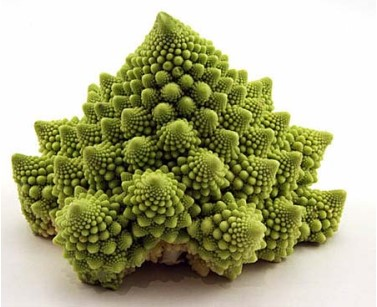
\includegraphics[scale=1]{../img/chou.jpg}\hspace{1cm}
\includegraphics[scale=1]{../img/fougere.jpg}
\end{center}

Si l'on ne regarde qu'une des pointes, on a l'impression de voir un chou en entier. C'est le principe
d'auto-similarité. On retrouve de l'auto-similarité dans les fougères (à droite) : chaque feuille ressemble à la fougère entière.


%\section*{La courbe du dragon}
%La courbe du dragon (ou « Fractale du dragon » ou « courbe de Heighway » ou « dragon de
%Heighway ») a été pour la première fois étudiée par les physiciens de la NASA John Heighway,
%Bruce Banks, et William Harter. Elle a été décrite par Martin Gardner dans sa chronique de jeux
%mathématiques du Scientific American en 1967. Nombre de ses propriétés ont été publiées par
%Chandler Davis et Donald Knuth.
%
%La courbe du dragon se construit ainsi:
%\begin{center}
%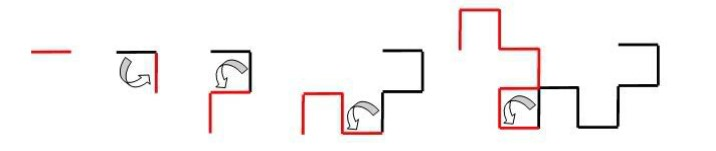
\includegraphics[scale=0.8]{../img/courbe_dragon.jpg}
%\end{center}
%
%\begin{itemize}
%\item Si n = 0, on dessine une ligne. C'est la base (ou l'initiateur). La longueur a peu
%d'importance. On définit la longueur une fois avec un paramètre.
%\item Sinon, si n > 0 :
%\begin{itemize}
%\item Dragon (n-1)
%\item On tourne à 90 degrés
%\item Dragon (n-1). 
%\end{itemize}
%C'est la règle de récursivité (ou le générateur).
%\end{itemize}
%
%\begin{enumerate}
%\item Programmer cette fractale pour la représenter avec le la librairie Turtle.
%\item Dessiner cette fractale. Que remarquez-vous ?
%\item Pour obtenir une fractale correcte, il faut introduire une rotation de -90 degrés. L'astuce consiste à passer un second paramètre s dans la fonction qui prendra comme valeur 1 ou -1 et on multiplie l'angle de rotation par s. Modifier votre programme en conséquence.
%
%La figure ci-dessous représente une fractale du dragon pour n=8.
%\begin{center}
%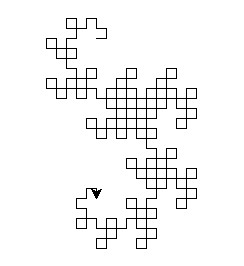
\includegraphics[scale=1]{../img/fractale_dragon.jpg}
%\end{center}
%\end{enumerate}

\section*{La courbe de von Koch}

La courbe de von Koch est l'une des premières courbes fractales à avoir été décrite (bien avant l'invention du terme « fractal(e) »). Elle a été inventée en 1906 par le mathématicien suédois Helge von Koch.

Cette courbe se réalise à partir d'un segment de droite de longueur $l$.

\begin{enumerate}
\item On divise le segment de droite en trois segments de longueurs égales $\dfrac{l}{3}$.
\item On dessine 4 segments de longueur $\dfrac{l}{3}$ en effectuant des rotations pour obtenir la forme pointue au centre.
\item on recommence le processus sur chacun des 4 morceaux de segments.
\end{enumerate}\medskip

\begin{center}
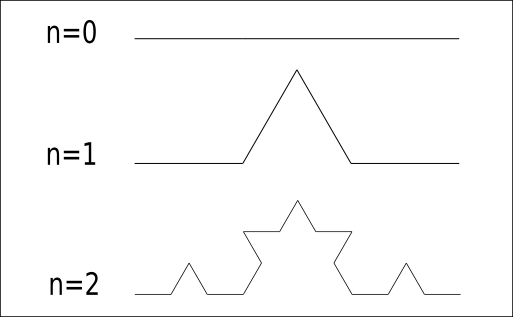
\includegraphics[scale=0.6]{../img/courbe_van_koch.png}
\end{center}


On donne la courbe de Von Koch pour trois valeurs de n. Le motif à reproduire est finalement celui obtenu avec $n=1$.

La courbe de Von Koch est la limite des courbes obtenues, lorsqu'on répète indéfiniment les étapes mentionnées ci-avant.


\begin{enumerate}
\item Importer dans un nouveau fichier Python le module turtle.
\item Écrire un code qui trace le motif de Von Koch obtenu pour $n=1$.
\item La fonction récursive \textsf{courbe\_von\_koch} de paramètres $l$ et $n$  trace la courbe de Von Koch pour un segment de longueur initiale égale à $l$.
\begin{itemize}
\item La condition d'arrêt vérifiée quand $n=0$ trace un segment de longueur $l$;
\item Si $n$ n'est pas égal à 1, on trace le motif de Von Koch en traçant les quatre segments de longueur $\dfrac{l}{3}$. Chaque tracé de segment est un appel récursif de la fonction.
\end{itemize}

\end{enumerate}

\section*{Les flocons de Von Koch}


Le \textbf{flocon de von Koch} s'obtient de la même façon que
la fractale précédente, en partant d'un triangle équilatéral
au lieu d'un segment de droite, et en effectuant les
modifications en orientant les triangles vers l'extérieur.

\begin{center}
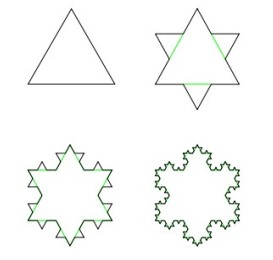
\includegraphics[scale=0.6]{../img/flocon_van_koch}
\end{center}

\begin{enumerate}
\item La fonction \textbf{courbe\_van\_koch(n,l)} prend en paramètre le nombre de répétitions du modèle obtenu lorsque n=1 et la longueur initiale $l$ du segment. Cette fonction dessine la courbe de Van Koch.
\item Écrire une fonction qui dessine le \textbf{flocon de Van Koch} à partir d'un triangle équilatéral.
\item Récrire vos deux fonctions en y apportant les modifications nécessaires pour que le modèle initial ressemble à la figure suivante:
\begin{center}
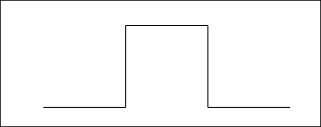
\includegraphics[scale=0.6]{../img/carre_van_koch.png}
\end{center}
\item Réaliser une fractale avec n=5.
\item Construire une figure superposant les fractales pour n=0 jusqu'à n=5 (figure ci-dessous).
\begin{center}
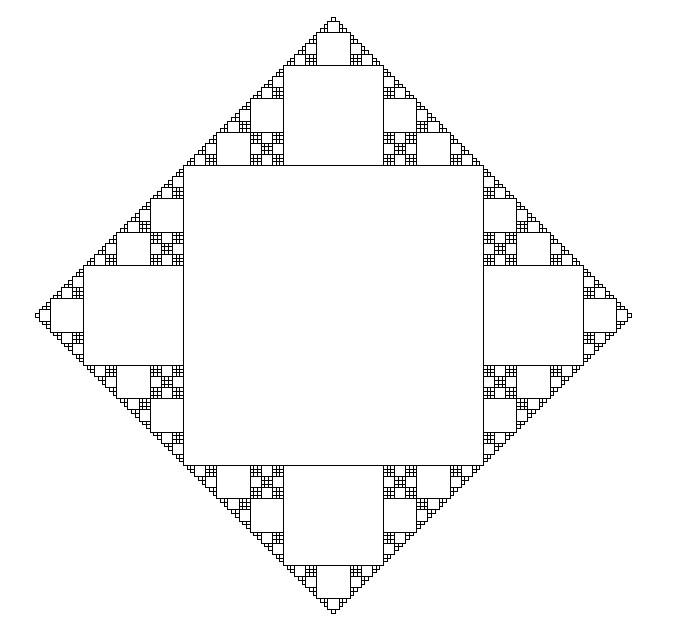
\includegraphics[scale=0.6]{../img/carre_fractale_5.jpg}
\end{center}
\end{enumerate}

\section*{L'arbre ou la fleur}

Le tracé d'un arbre ou d'une fleur peut être réalisé par une fractale.

La fractale florale représentée ci-dessous a un niveau de récursivité égal à 10 et une longueur initiale de 200.

\begin{center}
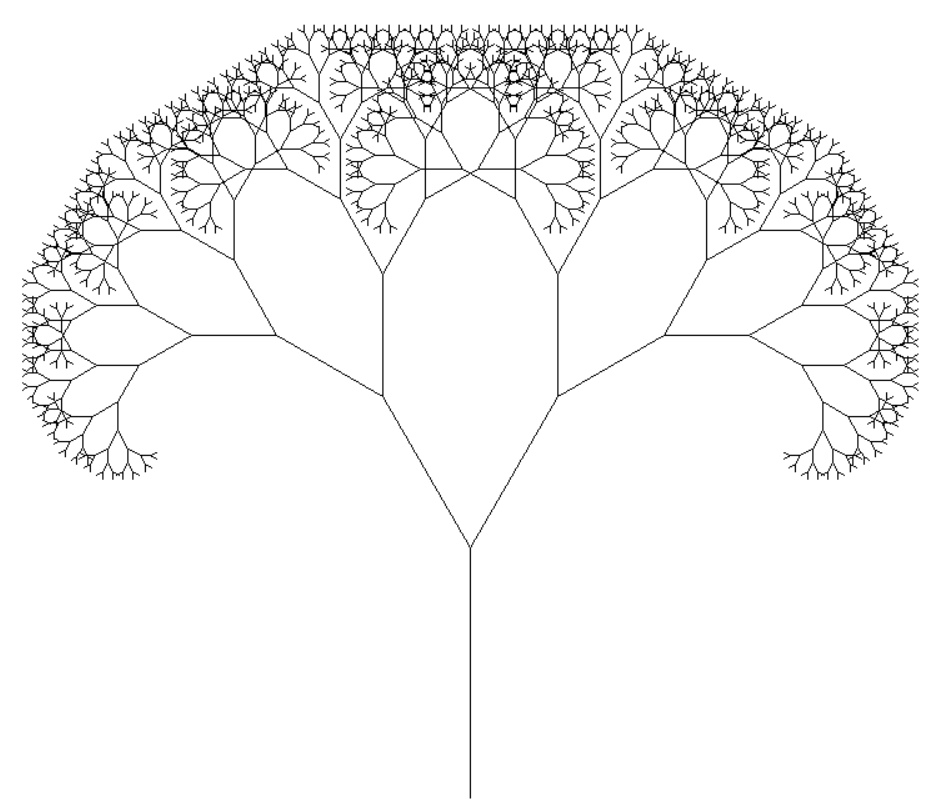
\includegraphics[scale=0.6]{../img/fleur_10_200}
\end{center}

Voici quelques indications :
\begin{itemize}
\item On remplace chaque segment par un motif en forme de Y.
\item Les angles de rotation pour tracer les branches sont de 30 degrés.
\item Chaque nouvelle branche a une longueur réduite égal à 70\% de la longueur du segment dont elle est issue.
\item Une fois le tracé d'un trait réalisé, il faut revenir en arrière avec la commande \textbf{backward()}
\end{itemize}


\begin{enumerate}
\item Importer dans un nouveau fichier Python le module turtle.
\item Écrire un code qui trace un motif en forme de Y.
\item La fonction récursive \textsf{arbre} de paramètres $n$ et $longueur$  trace la fleur pour un segment de longueur initiale égale à $longueur$.
\begin{itemize}
\item La condition d'arrêt vérifiée quand $n=0$ trace un segment de longueur $longueur$;
\item Si $n$ n'est pas égal à 1, on trace le motif en Y en traçant les branches par des appels récursifs à la fonction \textsf{arbre} en réduisant la valeur des paramètres.
\end{itemize}

\end{enumerate}


\end{document}
